\documentclass[exercice]{thedocument}%
\startdatakeys
    \source{originale}
    \BO{2026}
    \cycle{3}
    \competencesDuSocle{RE}
    \objectifsApprentissage{C3C2al,C3C2am}
    \motsCles{triangle, angles, construction géométrique}
\enddatakeys
\begin{document}%
    \begin{enumerate}
        \item Construire les bissectrices des trois angles du
        triangle ci dessous. Que remarques-tu~?
        \begin{center}
            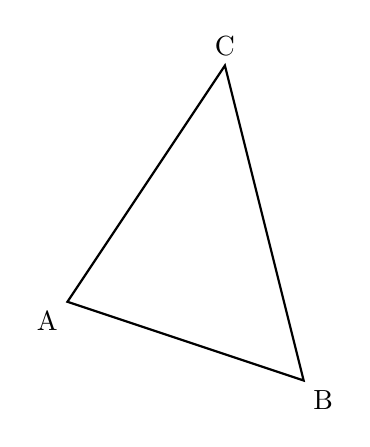
\begin{tikzpicture}[scale=1]
                \coordinate (A) at (0,0);
                \coordinate (B) at (3,-1);
                \coordinate (C) at (2,3);
                \draw[thick] (A) -- (B) -- (C) -- cycle;
                \node[below left] at (A) {A};
                \node[below right] at (B) {B};
                \node[above] at (C) {C};
            \end{tikzpicture}
        \end{center}
    \end{enumerate}
\end{document}